\documentclass[11pt]{article}

\usepackage[margin=1in]{geometry}                                              
\usepackage{amsmath,amsthm,amssymb}                                            
\usepackage{graphicx}                                      
\graphicspath{{../figures/}, {../figures/growthrates/}, {../figures/correlations/}, {../python/Hamiltonian/figures/}}
\usepackage{titlesec}                                                          
\usepackage{savetrees}                                                         
\usepackage{bm}

\titleformat{\subsection}[runin]
{\normalfont\large\bfseries}{\thesubsection}{1em}{}

\renewcommand{\bf}{\mathbf}
\renewcommand{\cal}{\mathcal}
\newcommand{\pd}[2]{\frac{\partial #1}{\partial #2}}
\newcommand{\pdn}[3]{\frac{\partial^{#3} #1}{\partial #2^{#3}}}
\newcommand{\pdop}[1]{\frac{\partial}{\partial #1}}
\newcommand{\nd}[2]{\frac{d #1}{d #2}}
\newcommand{\ndn}[3]{\frac{d^{#3} #1}{d #2^{#3}}}
\newcommand{\ndop}[1]{\frac{d}{d #1}}
\newcommand{\dt}{\frac{d}{dt}}
\newcommand{\grad}{\bm\nabla}
\newcommand{\cross}{\times}
\newcommand{\curl}{\grad\cross}
\newcommand{\imp}{\Longrightarrow\quad}
\newcommand{\abs}[1]{\left|#1\right|}
\newcommand{\half}{\frac{1}{2}}
\newcommand{\third}{\frac{1}{3}}
\renewcommand{\th}[1]{\frac{1}{#1}}
\renewcommand{\k}{4\pi\epsilon_0}
\newcommand{\eps}{\epsilon_0}
\newcommand{\intt}{\int_{t_1}^{t_2}}
\newcommand{\inti}{\int_{-\infty}^{+\infty}}
\newcommand{\ex}[1]{\left\langle #1 \right\rangle}
\newcommand{\oom}[1]{\times 10^{#1}}
\renewcommand{\d}{\delta}
\newcommand{\e}{\text{e}}
\renewcommand{\l}{\ell}
\newcommand{\om}{\omega}
\newcommand{\h}{\hbar}
\newcommand{\ket}[1]{\left|#1\right\rangle}
\newcommand{\bra}[1]{\left\langle#1\right|}
\newcommand{\braket}[2]{\left\langle#1\middle|#2\right\rangle}
\newcommand{\brakett}[3]{\left\langle#1\middle|#2\middle|#3\right\rangle}
\newcommand{\nn}{\nonumber\\}

\renewcommand{\thesection}{\arabic{section}:}
\renewcommand{\thesubsection}{(\alph{subsection})}

\begin{document}

\title{Thesis Update - Hamiltonian Behavior}
\author{Charles Stahl}

\maketitle

\section{Leading Edge Weight} \emph{}

The patterns from $L=9$ continue into $L=11$. For the forward-propagating wave, with $A(t=0)=Z_0$, the successive peaks fall off in size but dominate the Pauli strings until the last site takes over (figure~\ref{fig:L11end3n20front}). For the backward-propagating waves $(A(t=0)=Z_{L-1})$, the initial decaying signal is more difficult to make out but still present. It is dominated by a large weight of sites that start on site 9 around $t=1$. By $t = 3$ the first site has started to dominate the Pauli weights.

\begin{figure}
	\centering
	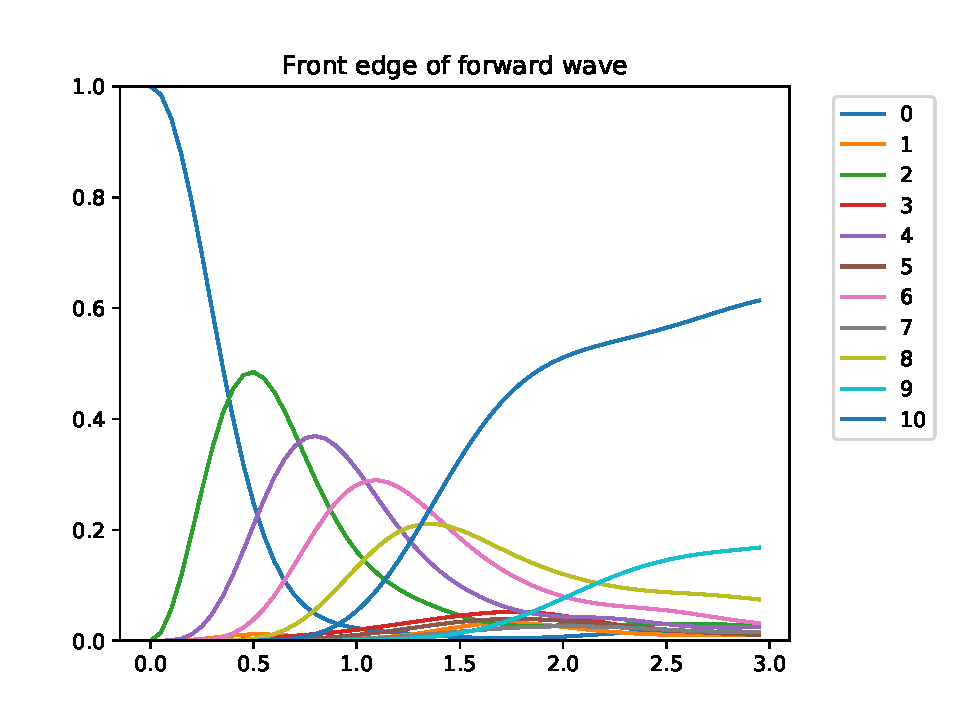
\includegraphics[width=.7\textwidth]{L11end3n20front}
	\caption{Weight of operators that end on site $i$.}
	\label{fig:L11end3n20front}
\end{figure}
\begin{figure}
	\centering
	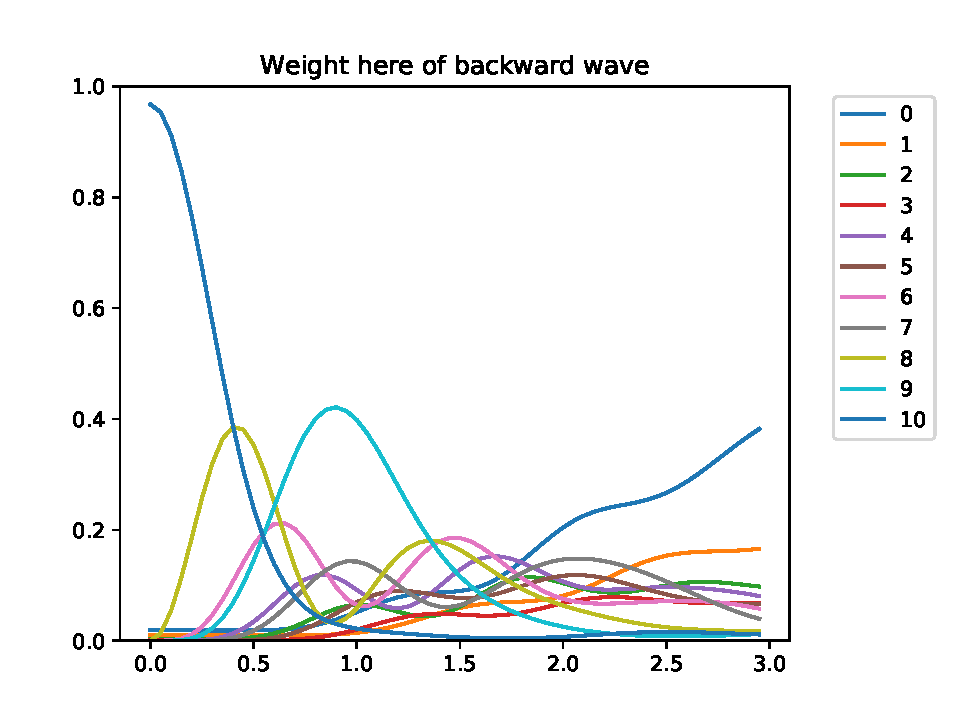
\includegraphics[width=.7\textwidth]{L11end3n20back}
	\caption{Weight of operators that begin on site $i$.}
	\label{fig:L11end3n20back}
\end{figure}

The initial behavior also matches the $L=9$ case. For forward propagation the initial behavior is $W(t;i) = a\e^{bt}$ with $a,b$ given by
\begin{align*}
\begin{tabular}{rll}
$i$ & $b$ & $a$\\
0 &-0.22806104 &-0.64537868\\
1 & 3.506984  &-0.7706456\\
2 & 1.81723584  &1.24814523\\
3 & 5.61941276 &-0.85107562\\
4 & 3.84629108  &1.71062193\\
5 & 7.69020229 &-1.63644758\\
6 & 5.8674097   &1.33960991\\
7 & 9.7051822  &-2.99655938\\
8 & 7.8830393   &0.37761653\\
9 & 11.6271597   &-4.90046795\\
10 & 9.88377179 &-1.04727877
\end{tabular}
\end{align*}
Figure~\ref{fig:L11end1n60fore} shows this behavior, while figure~\ref{fig:L11end1n60back} shows the analogous behavior for the backward propagating wave. 

\begin{figure}
	\centering
	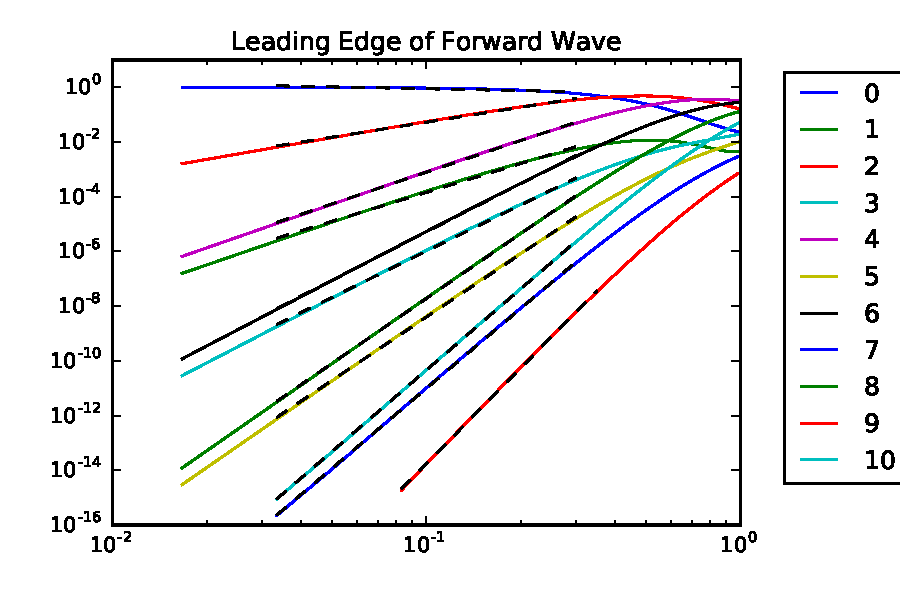
\includegraphics[width=.7\textwidth]{L11end1n60fore}
	\caption{Early-time leading edge weights for forward propagating wave.}
	\label{fig:L11end1n60fore}
\end{figure}
\begin{figure}
	\centering
	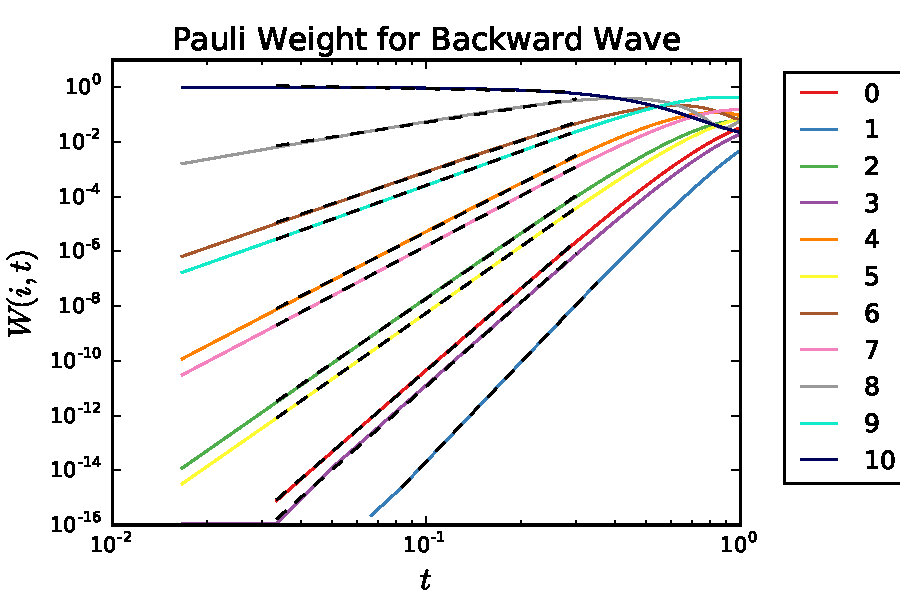
\includegraphics[width=.7\textwidth]{L11end1n60back}
	\caption{Early-time leading edge weights for backward propagating wave.}
	\label{fig:L11end1n60back}
\end{figure}

Here the relevant numbers are
\begin{align*}
\begin{tabular}{rll}
$i$ & $b$ & $a$\\
0 & 9.9088299  &-1.00930783\\
1 & 12.00638086 & -3.83892069\\
2  &7.87707656  &0.36158689\\
3  &10.17593682  &-1.72255575\\
4  &5.85872894  &1.31627132\\
5  &8.05004908 &-0.45346985\\
6  &3.83304312 & 1.67501865\\
7  &6.06924933 & 0.6277478 \\
8  &1.79673821 & 1.19312054\\
9  &4.12769107 & 1.25737669\\
10 &-0.22806104& -0.64537868
\end{tabular}
\end{align*}
Again, the exponents for even and odd sites increase by one within each group. Pairs of sites separated by 3 are also divergent in the forward case while convergent in the backward case.

\section{Weight at a Given Site}

If we look at the weight of non-identity operators at a site instead of weight of non-identity strings that end on a site, the behavior is more similar between even and odd sites. Figures~\ref{fig:L11end1n60_herefore} and~\ref{fig:L11end1n60_hereback} show the early behavior.
\begin{figure}
	\centering
	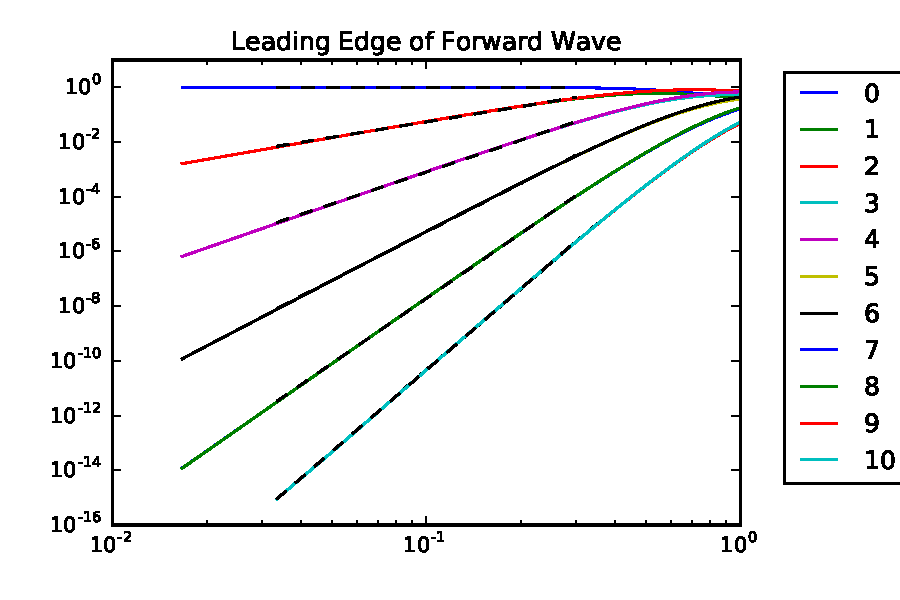
\includegraphics[width=.7\textwidth]{L11end1n60_herefore}
	\caption{Early-time weights at site $i$ for forward propagating wave.}
	\label{fig:L11end1n60_herefore}
\end{figure}
\begin{figure}
	\centering
	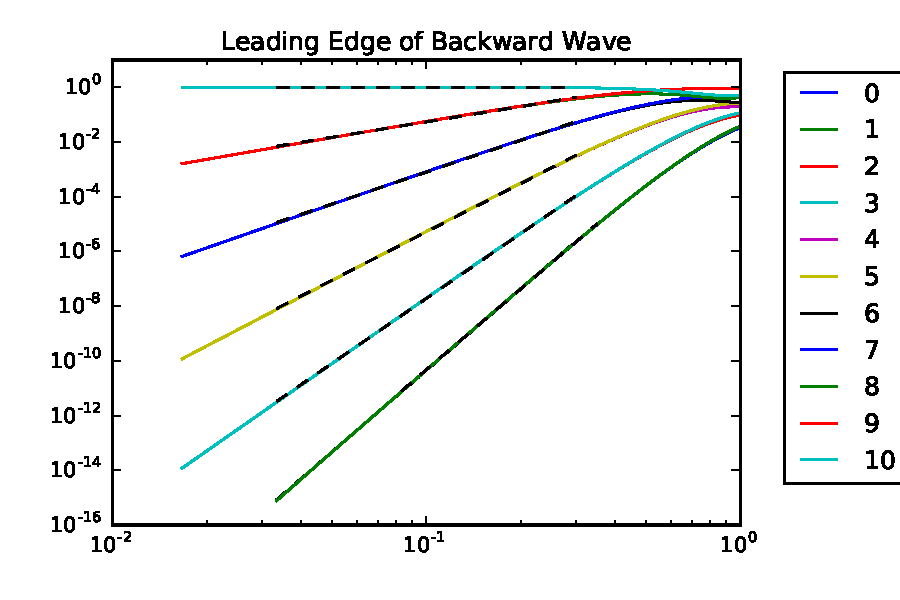
\includegraphics[width=.7\textwidth]{L11end1n60_hereback}
	\caption{Early-time weights at site $i$ for backward propagating wave.}
	\label{fig:L11end1n60_hereback}
\end{figure}
Now, the 2-site translational symmetry broken by triplet asymmetry is more visible. At early times, each pair of sites past the initial site is almost identical. The differences are not visible on the plot. The best fit parameters for forward propagation are 
\begin{align*}
\begin{tabular}{rll}
$i$ & $b$ & $a$\\
0 &-0.0110169 & -0.02903279\\
1 & 1.85885984&  1.36784057\\
2 & 1.87645224&  1.41529219\\
3 & 3.86681506&  1.76926911\\
4 & 3.87270585 & 1.78515861\\
5 & 5.87947281 & 1.37400747\\
6 & 5.88219513 & 1.38134381\\
7 & 7.8910584  & 0.40044216\\
8 & 7.89252802 & 0.40439999\\
9 & 9.80995422 &-1.17920962\\
10 & 9.88377179 &-1.04727877
\end{tabular}
\end{align*}
and for backward propagation are
\begin{align*}
\begin{tabular}{rll}
$i$ & $b$ & $a$\\
0 & 9.9088299 & -1.00930783\\
1 & 9.80392469& -1.1921265 \\
2 & 7.88661177&  0.38849071\\
4 & 5.87363142&  1.35830824\\
5 & 5.87665983&  1.36644734\\
6 & 3.8665327 &  1.76853724\\
8 & 1.85741308&  1.36404258\\
9 & 1.87784882&  1.41896213\\
10 &-0.0110169&  -0.02903279\\
\end{tabular}
\end{align*}

Figures~\ref{fig:L11end3n20_herefront} and~\ref{fig:L11end3n20_hereback} show their evolution at later time. In both cases, in all pairs, the odd site eventually overtakes the even site, pointing out the asymmetry in the triplets.
\begin{figure}
	\centering
	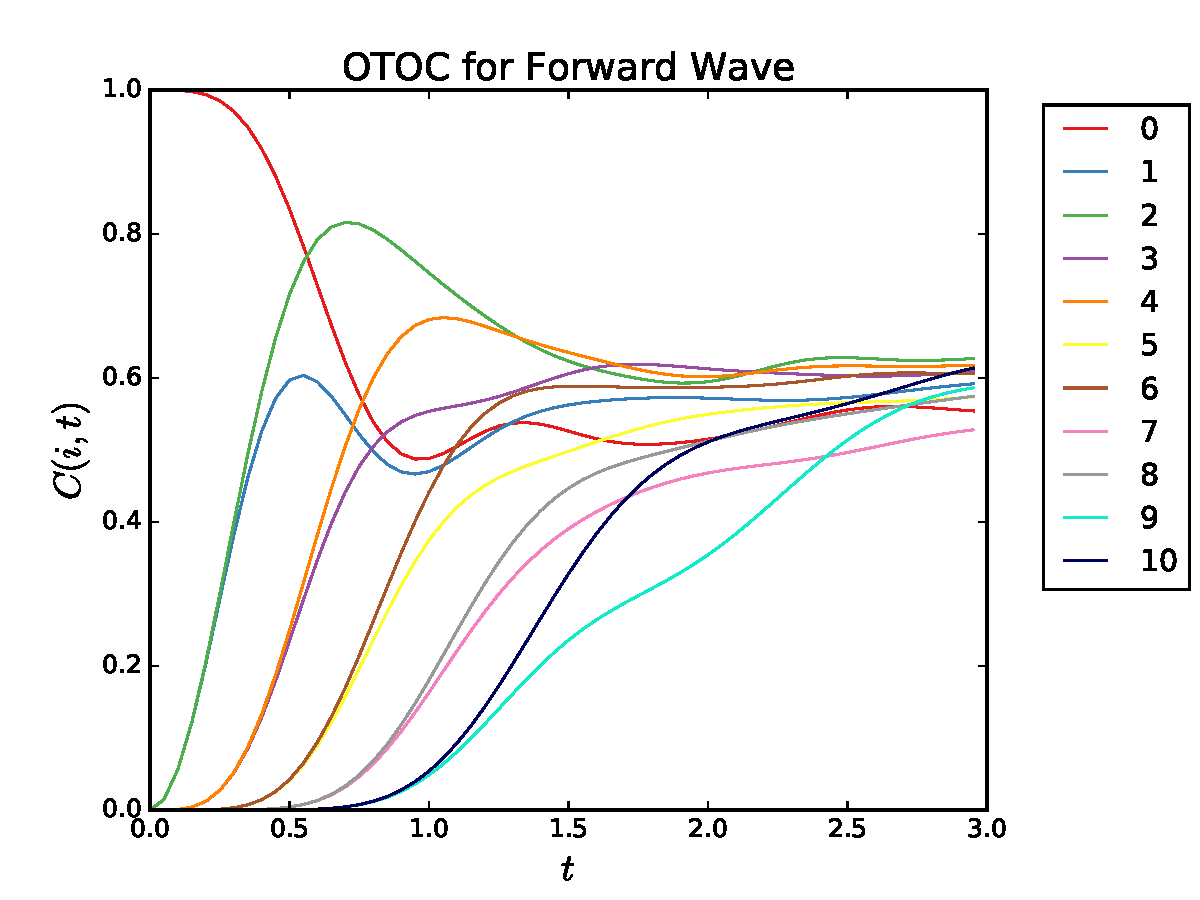
\includegraphics[width=.7\linewidth]{L11end3n20_herefront}
	\caption{Weight of non-identity operators at site $i$.}
	\label{fig:L11end3n20_herefront}
\end{figure}
\begin{figure}
	\centering
	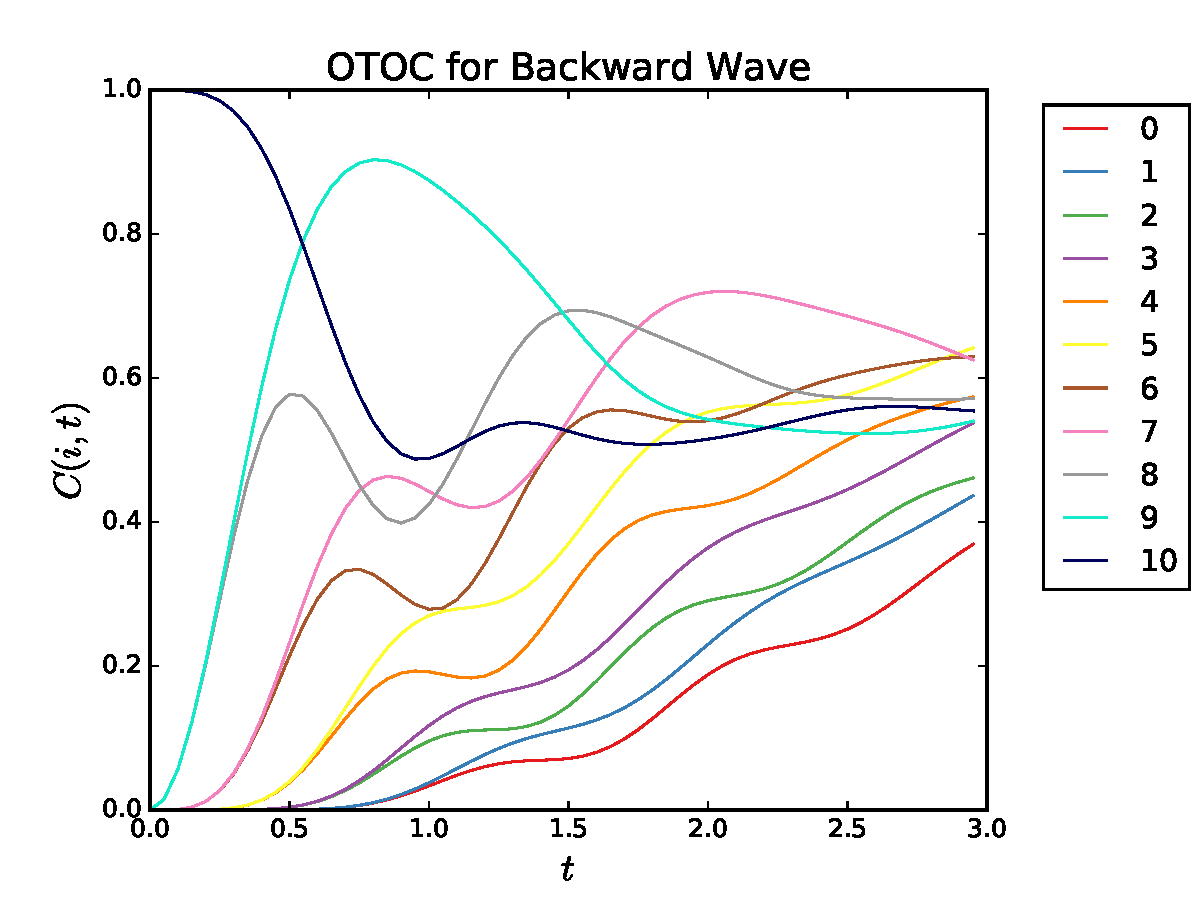
\includegraphics[width=.7\linewidth]{L11end3n20_hereback}
	\caption{Weight of non-identity operators at site $i$.}
	\label{fig:L11end3n20_hereback}
\end{figure}

\end{document}
